\chapter{Interprocess Communication - Implementation \& Design}
There are many possible kinds of communications, so we will illustrate the three most important
\begin{itemize}
    \item \textbf{Socket:}
        \begin{itemize}
            \item Creates a \textbf{channel} at low level between processes on different hosts
            \item In which for each application it is necessary to define a \textbf{protocol for data coding and decoding}
            \item This solution implements a \textbf{lack of transparency}
        \end{itemize}
    \item \textbf{Remote Procedure Call or RPC:} allows client programs to call procedures transparently in server programs running in separate processes. More deeply:
        \begin{itemize}
            \item There is an \textbf{abstraction} of the process communication at a level of procedure call
            \item The parameters are \textbf{packed and sent} to the destination after the encoding
            \item Data \textbf{conversion} between different supports introduces a very \textbf{high overhead}
            \item It is connected to the \textbf{process definition} and it cannot be integrated in the Object Oriented code
        \end{itemize}
    \item \textbf{Remote Method Invocation or RMI:}
        \begin{itemize}
            \item Allows an application running on a local machine to invoke the methods of another application running on a remote machine
            \item Locally only a \textbf{remote object reference} is created, that is actually active on a different host
            \item All the invocation of the methods to be transmitted are handled by the \textbf{Object Remote Broker (ORB)}
        \end{itemize}
\end{itemize}
Middleware provides transparency to the interprocess communication:

\section{UDP}
UDP represents a \textbf{datagram communication without ordering and reliability.} 
\begin{itemize}
    \item Interface to UDP is based on \textbf{message passing} to enable sending a single message from sender to receiver
    \item Communication procedure is based like so:
        \begin{itemize}
            \item \textbf{Client} (sender or receiver):
                \begin{itemize}
                    \item Create socket
                    \item Link it to the IP address and port Server
                \end{itemize}
            \item \textbf{Server:}
                \begin{itemize}
                    \item Create socket
                    \item Link it to a port
                    \item Link the clients know the port 
                \end{itemize}
            \item There can be many type of \textbf{failure like:}
                \begin{itemize}
                    \item \textbf{Omission:} lost of message (channel fault, checksum, limited space)
                    \item \textbf{Arbitrary:} unordered delivery
                \end{itemize}
        \end{itemize}
\end{itemize}
Moreover the communication procedure in JAVA UDP is formed by two clases:
\begin{itemize}
    \item \textbf{DatagramPacket:} which for the actual transmitted packet formed as so:
    
    \begin{figure}[!h]
    \centering
    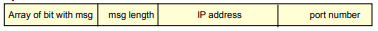
\includegraphics[width=.7\linewidth]{images/InterprocessCommunicationImplementationDesign/datagrampacket.png}
    \caption{DatagramPacket components}
\end{figure}
    
    \item \textbf{DatagramSocket:} which provides the number of the port to a process that asks for it allowing the system to choose a free port
\end{itemize}
For sending and receiving there are three methods to extract the information:
\begin{itemize}
    \item gatPort
    \item getData
    \item getAddress
\end{itemize}

\begin{figure}[!h]
    \centering
    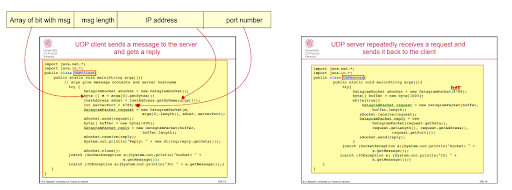
\includegraphics[width=.9\linewidth]{images/InterprocessCommunicationImplementationDesign/datagramjava.png}
    \caption{Java Datagram Application}
\end{figure}
\newpage

\section{TCP}
TCP opens a \textbf{stream of communication}
\begin{itemize}
    \item Interfaces to TCP are based on \textbf{bidirectional stream} and to enable \textbf{sending a stream of data} between sender and receiver
    \item It is based on \textbf{producer-consumer communication}
    \item In TCP the destination is the couple (IP address, port number), so the \textbf{server} has to let the client \textbf{know} this \textbf{couple of data}
        \begin{itemize}
            \item This means there is a \textbf{lack of transparency}
                \begin{itemize}
                    \item It could be solved by referencing to the service by name and using a \textbf{name server}
                    \item Moreover the server OS provides the name so that there is \textbf{location independence = location transparency + migration transparency}
                \end{itemize}
        \end{itemize}
    \item The communication in TCP is based like so:
        \begin{itemize}
            \item \textbf{Client:}
                \begin{itemize}
                    \item Create stream socket
                    \item Link it to any port
                    \item Execute a connect
                \end{itemize}
            \item \textbf{Server:}
                \begin{itemize}
                    \item Create a listen socket
                    \item Link to a port
                    \item Wait for a connect request \(\rightarrow\) queue
                    \item Execute an \textbf{accept} by creating a \textbf{stream socket} for that client and keep the other port free to listen to other
                \end{itemize}
        \end{itemize}
        \newpage
        \item There can be different \textbf{failure} also in TCP:
            \begin{itemize}
                \item Possible block due to the buffer of the destination socket, control of the correctness, duplication and ordering, control of the message loss
                \item The \textbf{Failure Model} to ensure these types of error is
                    \begin{itemize}
                        \item Control of the correctness, duplication, ordering and control of the message loss
                    \end{itemize}
            \end{itemize}
\end{itemize}